%
% IMS Conference Sample Paper
% 
% HISTORY
% 20180920 V3 first release for review
% 20180924 V3b minor text changes regarding hiding text for blind review
% 20181009 V3c - boldfaced the warning to not use old papers as templates
%              - increased fig 1 size
%              - changed example keywords for RFIC
% 20191020 V4c - TPC supplied new text with added emphasis concerning the process
%                of preparing papers for double-blind peer review.
%              - tiny adjustment of side margins
%              - developed strategy for using template with XeTeX/LuaTeX and pdfLaTeX to
%                in recent TeXLive installations
%              - replaced fig 1 with new graph
%              - replaced fig 2 with new IC die photos
%              - added Figure Label (eg (a) (b) for subfigures) font spec to table 1
%              - minor formatting changes
%              - minor text changes
% 20201028 V5  - IMS has changed page limits to 3 pages total maximum for initial submissions for 
%                review, and 4 pages maximum for final submissions where the 4th page if present
%                must contain only references.
% 20220823 V6 - IMS has changed page limits to 3 pages minimum and 4 pages total maximum,
%.               for both paper review and final version.  For authors submitting final paper to MWTL
%                Special Issue, the second column on the final page may only contain an 
%                acknowledgement and references.   
%%%%%%%%%%%%%%%%%%%%%%%%%%%%%%%%%%%%%%%%%%%%%%%%%%%%%%%%%%%%%%%%%%%%%%%%%%%%%
% We first setup margins for IMS papers on USL paper.  This is done 
% before the \documentclass is invoked.
%
\newcommand{\CLASSINPUTtoptextmargin}{0.75in}%
\newcommand{\CLASSINPUTbottomtextmargin}{1in}%
\newcommand{\CLASSINPUTinnersidemargin}{0.63in}%
\newcommand{\CLASSINPUToutersidemargin}{0.63in}%
%
%%%%%%%%%%%%%%%%%%%%%%%%%%%%%%%%%%%%%%%%%%%%%%%%%%%%%%%%%%%%%%%%%%%%%%%%%%%%%
%
% requires IEEEtran V1.8+, as hosted on CTAN at the following URL:
%	http://www.ctan.org/tex-archive/macros/latex/contrib/IEEEtran/
%
\documentclass[conference,10pt,letterpaper]{IEEEtran}% 
%
%%%%%%%%%%%%%%%%%%%%%%%%%%%%%%%%%%%%%%%%%%%%%%%%%%%%%%%%%%%%%%%%%%%%%%%%%%%%%
% Now we import required packages
%
\usepackage{amsmath}% for double integral symbol in this template
\usepackage{graphicx}% for figures
\usepackage{multirow}% to allow multiple-row elements in tabular environment
\usepackage[none]{hyphenat}% turn off hyphenation to make text extraction and indexing easier
\usepackage{float}% better control of floating figures and tables
\usepackage{subfig}% for subfigures within figures
\usepackage{dblfloatfix}% fix to allow page-wide floats at bottom of page
%%%%%%%%%%%%%%%%%%%%%%%%%%%%%%%%%%%%%%%%%%%%%%%%%%%%%%%%%%%%%%%%%%%%%%%%%%%%%
% users of pdfLaTeX must uncomment the following lines:
\usepackage{t1enc}% allows access to various special characters
\usepackage{times}% change font to Nimbus Roman (based on Times Roman)
%%%%%%%%%%%%%%%%%%%%%%%%%%%%%%%%%%%%%%%%%%%%%%%%%%%%%%%%%%%%%%%%%%%%%%%%%%%%%
% users of XeLaTeX or LuaTeX must uncomment the following two lines:
% \usepackage{fontspec}% needed to change main font
% \setmainfont{TeX Gyre Termes}% change font to TeX Gyre Roman (based on Times Roman)
%%%%%%%%%%%%%%%%%%%%%%%%%%%%%%%%%%%%%%%%%%%%%%%%%%%%%%%%%%%%%%%%%%%%%%%%%%%%%
%
%%%%%%%%%%%%%%%%%%%%%%%%%%%%%%%%%%%%%%%%%%%%%%%%%%%%%%%%%%%%%%%%%%%%%%%%%%%%%
% Next we modify the standard IEEEtran.cls format to produce IMS format by 
% redefining some macros.
% IMS_modify_IEEEtran_18b_CTAN_V5.tex
%         created by Causal Productions Pty Ltd, 
%	  http://www.causalproductions.com
%	  info@causalproductions.com
%
%	  This file is Copyright 2017-2019 Causal Productions Pty Ltd.
%	  Permission is granted to use this file and its associated files
%	  for conferences for which Causal Productions has been contracted
%	  to prepare the conference proceedings.
%
% This file contains format modifications to the standard IEEE style file
% called IEEEtran.cls version 1.8b, as hosted on CTAN at the following URL:
%	http://www.ctan.org/tex-archive/macros/latex/contrib/IEEEtran/
%
% The purpose of the format modifications is to implement a paper format
% traditionally used by IMS conferences, which differs from the standard
% IEEE conference paper format in various ways, such as font sizes.
%  
% This file is NOT intended to be used with the different IEEEtran.cls version 1.8
% that is distributed by IEEE at the following URL:
%	http://www.ieee.org/web/publications/pubservices/confpub/AuthorTools/conferenceTemplates.html
% Despite having the same version number 1.8, the CTAN and IEEE versions are
% different and this particular modification file is designed only for the 
% CTAN version.
%
% HISTORY
% 20180920 V3 first release for review
% 20181009 V3c no change, version number bumped to match paper template file
% 20191020 V4c changed section heading number-name spacing so that it is specified individually for
%               section - use a fixed space between number and name
%               subsection - make the name align with paragraph indentation
%               subsubsection - make the name align with paragraph indentation
%               paragraph - make the name align with paragraph indentation
% 20201028 V5 no change, version number bumped to match paper template file
% 20220823 V6 no change, version number bumped to match paper template file
%%%%%%%%%%%%%%%%%%%%%%%%%%%%%%%%%%%%%%%%%
\makeatletter

\def\@IMSauthorblockNAMEstyle{\normalfont\IMSauthorsize}
\def\@IMSauthorblockAFFILstyle{\normalfont\IMSaffilsize}
\def\@IMSauthorblockEMAILstyle{\normalfont\IMSaffilsize}
%
\def\IMSauthorblockNAME#1{%
\relax\@IMSauthorblockNAMEstyle%
#1%
}%
\def\IMSauthorblockAFFIL#1{%
\relax\@IMSauthorblockAFFILstyle%
\vskip\@IEEEauthorblockAtopspace
#1%
}%
\def\IMSauthorblockEMAIL#1{%
\relax\@IMSauthorblockEMAILstyle%
\vskip\@IEEEauthorblockAtopspace
#1%
}%
%
\newcommand{\IMSauthor}[1]{%
\ifIsBlindReviewVersion%
\author{\phantom{\parbox{\textwidth}{\center\relax#1}}}%
\else%
\author{\parbox{\textwidth}{\center\relax#1}}%
\fi%
}%
%
\newif\ifIsBlindReviewVersion
\def\IMSthispaperforblindreview{\IsBlindReviewVersiontrue}
\def\IMSthispaperforfinalpublication{\IsBlindReviewVersionfalse}
%
%
%
% IMS: override title block font sizes
% formats the Title, authors names, affiliations and special paper notice
% THIS IS A CONTROLLED SPACING COMMAND! Do not allow blank lines or unintentional
% spaces to enter the definition - use % at the end of each line
\def\@maketitle{\newpage
\bgroup\par\addvspace{0.5\baselineskip}\centering%
\ifCLASSOPTIONtechnote% technotes
   {\bfseries\large\@IEEEcompsoconly{\sffamily}\@title\par}\vskip 1.3em{\lineskip .5em\@IEEEcompsoconly{\sffamily}\@author
   \@IEEEspecialpapernotice\par{\@IEEEcompsoconly{\vskip 1.5em\relax
   \@IEEEtitleabstractindextextbox{\@IEEEtitleabstractindextext}\par
   \hfill\@IEEEcompsocdiamondline\hfill\hbox{}\par}}}\relax
\else% not a technote
   \vskip0.2em{\IMStitlesize\ifCLASSOPTIONtransmag\bfseries\LARGE\fi\@IEEEcompsoconly{\sffamily}\@IEEEcompsocconfonly{\normalfont\normalsize\vskip 2\@IEEEnormalsizeunitybaselineskip
   \bfseries\Large}\@title\par}\vskip1.0em\par% CAUSAL PRODUCTIONS change on this line
   % V1.6 handle \author differently if in conference mode
   \ifCLASSOPTIONconference%
      {\@IEEEspecialpapernotice\mbox{}\vskip\@IEEEauthorblockconfadjspace%
       \mbox{}\hfill\begin{@IEEEauthorhalign}\@author\end{@IEEEauthorhalign}\hfill\mbox{}\par}\relax
   \else% peerreviewca, peerreview or journal
      \ifCLASSOPTIONpeerreviewca
         % peerreviewca handles author names just like conference mode
         {\@IEEEcompsoconly{\sffamily}\@IEEEspecialpapernotice\mbox{}\vskip\@IEEEauthorblockconfadjspace%
          \mbox{}\hfill\begin{@IEEEauthorhalign}\@author\end{@IEEEauthorhalign}\hfill\mbox{}\par
          {\@IEEEcompsoconly{\vskip 1.5em\relax
           \@IEEEtitleabstractindextextbox{\@IEEEtitleabstractindextext}\par\hfill
           \@IEEEcompsocdiamondline\hfill\hbox{}\par}}}\relax
      \else% journal, peerreview or transmag
         \ifCLASSOPTIONtransmag
            % transmag also handles author names just like conference mode
            % it also uses \@IEEEtitleabstractindextex, but with one line less
            % space above, and one more below
           {\@IEEEspecialpapernotice\mbox{}\vskip\@IEEEauthorblockconfadjspace%
            \mbox{}\hfill\begin{@IEEEauthorhalign}\@author\end{@IEEEauthorhalign}\hfill\mbox{}\par
           {\vspace{0.5\baselineskip}\relax\@IEEEtitleabstractindextextbox{\@IEEEtitleabstractindextext}\vspace{-1\baselineskip}\par}}\relax
         \else% journal or peerreview
           {\lineskip.5em\@IEEEcompsoconly{\sffamily}\sublargesize\@author\@IEEEspecialpapernotice\par
           {\@IEEEcompsoconly{\vskip 1.5em\relax
            \@IEEEtitleabstractindextextbox{\@IEEEtitleabstractindextext}\par\hfill
            \@IEEEcompsocdiamondline\hfill\hbox{}\par}}}\relax
         \fi
      \fi
   \fi
\fi\par\addvspace{0.0\baselineskip}\egroup}% CAUSAL PRODUCTIONS change on this line, reduce the vspace from 0.5\baselineskip to 0.0

% IMS: change font sizes in the document
%	paper title is 24pt
%	bib items are 9pt 
%	author names are 11pt
%	author affils are 10pt
%	captions of figs and tables are 9pt
\def\IMStitlesize{\@setfontsize{\IMStitlesize}{18}{21pt}}% CAUSAL PRODUCTIONS change on this line
\def\IMSauthorsize{\@setfontsize{\IMSauthorsize}{12}{13pt}}% CAUSAL PRODUCTIONS change on this line
\def\IMSaffilsize{\@setfontsize{\IMSaffilsize}{12}{13pt}}% CAUSAL PRODUCTIONS change on this line
\def\IMScaptionsize{\@setfontsize{\IMScaptionsize}{8}{9pt}}% CAUSAL PRODUCTIONS change on this line
\def\IMSbibsize{\@setfontsize{\IMSbibsize}{8}{9pt}}% CAUSAL PRODUCTIONS change on this line

\def\@IEEEauthorblockNstyle{\IMSauthorsize\@IEEEcompsocnotconfonly{\sffamily}\@IEEEcompsocconfonly{\large}}%CAUSAL PRODUCTIONS removed sublargesize to get correct IMSauthorsize
\def\@IEEEauthorblockAstyle{\IMSaffilsize\@IEEEcompsocnotconfonly{\sffamily}\@IEEEcompsocconfonly{\itshape}\@IEEEcompsocconfonly{\large}}%CAUSAL PRODUCTIONS removed normalsize to get correct IMSaffilsize
% The default if the user does not use an author block
\def\@IEEEauthordefaulttextstyle{\IMSauthorsize\@IEEEcompsocnotconfonly{\sffamily}\sublargesize}%CAUSAL PRODUCTIONS

\def\thebibliography#1{\section*{\refname}%
    \addcontentsline{toc}{section}{\refname}%
    % V1.6 add some rubber space here and provide a command trigger
    \IMSbibsize\@IEEEcompsocconfonly{\small}\vskip 0.3\baselineskip plus 0.1\baselineskip minus 0.1\baselineskip% CAUSAL PRODUCTIONS change on this line
    \list{\@biblabel{\@arabic\c@enumiv}}%
    {\settowidth\labelwidth{\@biblabel{#1}}%
    \leftmargin\labelwidth
    \advance\leftmargin\labelsep\relax
    \itemsep \IEEEbibitemsep\relax
    \usecounter{enumiv}%
    \let\p@enumiv\@empty
    \renewcommand\theenumiv{\@arabic\c@enumiv}}%
    \let\@IEEElatexbibitem\bibitem%
    \def\bibitem{\@IEEEbibitemprefix\@IEEElatexbibitem}%
\def\newblock{\hskip .11em plus .33em minus .07em}%
% originally:
%   \sloppy\clubpenalty4000\widowpenalty4000%
% by adding the \interlinepenalty here, we make it more
% difficult, but not impossible, for LaTeX to break within a reference.
% IEEE almost never breaks a reference (but they do it more often with
% technotes). You may get an underfull vbox warning around the bibliography, 
% but the final result will be much more like what IEEE will publish. 
% MDS 11/2000
\ifCLASSOPTIONtechnote\sloppy\clubpenalty4000\widowpenalty4000\interlinepenalty100%
\else\sloppy\clubpenalty4000\widowpenalty4000\interlinepenalty500\fi%
    \sfcode`\.=1000\relax}

% IMS: make a version of \@makecaption which uses \IMScaptionsize
%	and which formats all figure captions as justified if long, centered if short,
%	and formats all table captions using identical format to figure captions.
%	We are discarding the archaic small-caps format of table captions which was so hard to read.
%
\long\def\@makecaption#1#2{%
% test if is a for a figure or table
%  if figure, must make a vertical space before caption to separate caption from figure content
%  if table, must make a vertical space after caption to separate caption from table content
\ifx\@captype\@IEEEtablestring%
\par\@IEEEtabletopskipstrut% strut used to align table caption with facing column
\else
\@IEEEfigurecaptionsepspace
\fi
% 20180920 use IMScaptionsize, use two nonbreaking spaces, not one
\setbox\@tempboxa\hbox{\normalfont\IMScaptionsize {#1.}\nobreakspace\nobreakspace #2}%
\ifdim \wd\@tempboxa >\hsize%
% if caption is longer than a line, let it wrap around
\setbox\@tempboxa\hbox{\normalfont\IMScaptionsize {#1.}\nobreakspace\nobreakspace}%
\parbox[t]{\hsize}{\normalfont\IMScaptionsize\noindent\unhbox\@tempboxa#2}%
% if caption is shorter than a line, center if conference, left justify otherwise
\else
\ifCLASSOPTIONconference \hbox to\hsize{\normalfont\IMScaptionsize\hfil\box\@tempboxa\hfil}%
\else \hbox to\hsize{\normalfont\IMScaptionsize\box\@tempboxa\hfil}%
\fi\fi
% test if is a for a figure or table
%  if figure, must make a vertical space before caption to separate caption from figure content
%  if table, must make a vertical space after caption to separate caption from table content
\ifx\@captype\@IEEEtablestring%
\@IEEEtablecaptionsepspace
\else
\fi}

% IMS: define table-caption-to-table separation separately from figure-to-figure-caption separation
\newlength\tablecaptiontotableskip
\newlength\figuretocaptionskip
% but only \abovecaptionskip is used above figure captions and *below* table
% captions
\setlength\tablecaptiontotableskip{0.5\baselineskip}% 0.5bs gives about 3mm from caption baseline to table
\setlength\figuretocaptionskip{0.0\baselineskip}% 0bs gives about 3mm from figure to caption top of lc letters, which matches appearance of table.
\def\@IEEEfigurecaptionsepspace{\vskip\figuretocaptionskip\relax}%
\def\@IEEEtablecaptionsepspace{\vskip\tablecaptiontotableskip\relax}%

% IMS: Use Michael Shells suggested fix to reduce the space around emdash following Abstract and Index Terms headings
\def\abstract{\normalfont%
\@IEEEabskeysecsize\bfseries\textit{\abstractname}\,\bfseries\textit{---}\,%
\@IEEEgobbleleadPARNLSP}%
\def\endabstract{\relax\vspace{0ex}\par%
\normalfont\normalsize}%

\def\IEEEkeywords{\normalfont%
\@IEEEabskeysecsize\bfseries\textit{\IEEEkeywordsname}\,\bfseries\textit{---}\,%
\@IEEEgobbleleadPARNLSP}%
\def\endIEEEkeywords{\relax\vspace{0.67ex}%
\par\if@twocolumn\else\endquotation\fi%
\normalsize\normalfont}%


%%%%%
% Define \IMSauthorrefmark to allow more flexible marking than the \IEEEauthorrefmark command
% The refmarks can now be a string of any length, of any characters.
\DeclareRobustCommand*{\IMSauthorrefmark}[1]{\raisebox{0pt}[0pt][0pt]{\textsuperscript{\footnotesize{#1}}}}%
%
% CAUSAL PRODUCTIONS: No extra space between title and authors
\def\@IEEEauthorblockNtopspace{0ex}
% CAUSAL PRODUCTIONS: 1mm extra space between author names and affiliations
\def\@IEEEauthorblockAtopspace{1mm}
%
%%%%%%%%%%%%%%%%%%%%%%
%
\setlength{\columnsep}{6.3mm}% IMS
\def\tablename{Table}% IMS: was TABLE in IEEETran, but we are now using capitalized caption text not smallcaps
\def\thetable{\arabic{table}}% IMS: Tables are numbered using arabic not roman
\def\IEEEkeywordsname{Keywords}% use Keywords instead of Index Terms
%
%%%%%%%%%%%%%%%%%%%%%%
%
\def\subsubsection{\@startsection{subsubsection}{3}{\z@}{1.5ex plus 1.5ex minus 0.5ex}%
{0.7ex plus .5ex minus 0ex}{\normalfont\normalsize\itshape}}%
%
%%%%%%%%%%%%%%%%%%%%%%
%
\setlength{\parindent}{1.5em}% make the default para indent larger to match WORD template
%
% 20191023 we remove the V3c indentation of section headings to match paragraph indentation, 
% and revert to the original IEEE section heading style without spacing, and the spacing is
% now done individually for the 4 levels, below.
\def\@seccntformat#1{\csname the#1dis\endcsname\relax}% moved the spacer \hskip 0.5em to individual handlers below
%
% The following are copied from IEEEtran.cls line 2585 and modified here
\def\thesectiondis{\thesection.\hskip 0.5em}%					I.	% CAUSAL PRODUCTIONS: moved the hskip spacer from \@seccntformat to here
\def\thesubsectiondis{{\hbox to\parindent{\Alph{subsection}.}}}%		B.	% CAUSAL PRODUCTIONS: indent the subsection name to match paragraph indent
\def\thesubsubsectiondis{{\hbox to \parindent{\arabic{subsubsection})}}}%	3)	% CAUSAL PRODUCTIONS: indent the subsubsection name to match paragraph indent
\def\theparagraphdis{{\hbox to \parindent{\alph{paragraph})}}}%			d)	% CAUSAL PRODUCTIONS: indent the subsubsubsection name to match paragraph indent
%
% now we redefine the list indents so they take the new value of \parindent
\IEEEilabelindentA \parindent
\IEEEilabelindent \IEEEilabelindentA
\IEEEelabelindent \parindent
\IEEEdlabelindent \parindent
\IEEElabelindent \parindent
%%%%%%%%%%%%%%%%%%%%%%

\newlength\@IMSparindent
\setlength{\@IMSparindent}{\parindent}

\newcommand\IMSdisplayacksection[1]{%
\ifIsBlindReviewVersion%
%\noindent\phantom{\parbox[t]{\columnwidth}{\normalbaselines\setlength{\parindent}{\@IMSparindent}#1\strut}}%\IMSacktext
\noindent\phantom{\parbox[t]{\columnwidth}{\normalbaselines\setlength{\parindent}{\@IMSparindent}{#1}\strut}}%\IMSacktext
\else%
\noindent\parbox[t]{\columnwidth}{\normalbaselines\setlength{\parindent}{\@IMSparindent}{#1}\strut}%
\fi%
}%

%%%%%%%%%%%%%%%%%%%%%%

\makeatother


%%%%%%%%%%%%%%%%%%%%%%%%%%%%%%%%%%%%%%%%%%%%%%%%%%%%%%%%%%%%%%%%%%%%%%%%%%%%%
%
\newcommand{\IMSeventname}{IMS}% or RFIC or IMS
%
%%%%%%%%%%%%%%%%%%%%%%%%%%%%%%%%%%%%%%%%%%%%%%%%%%%%%%%%%%%%%%%%%%%%%%%%%%%%%
\begin{document}
%%%%%%%%%%%%%%%%%%%%%%%%%%%%%%%%%%%%%%%%%%%%%%%%%%%%%%%%%%%%%%%%%%%%%%%%%%%%%
% We use \raggedbottom to avoid latex adding vertical space around headings.
% This gives a better idea to the author about how much white space remains
% as the page limit is approached.
\raggedbottom
%
%%%%%%%%%%%%%%%%%%%%%%%%%%%%%%%%%%%%%%%%%%%%%%%%%%%%%%%%%%%%%%%%%%%%%%%%%%%%%
% PAPER TITLE AND AUTHOR BLOCK
%
% The paper title can use linebreaks \\ within to get better formatting if desired.
%
\title{\IMSeventname\ Template V6 in US Letter Page Size}
%
% Next we define the author names and affiliations.
% Author names are listed using \IMSauthorblockNAME{} with comma separators between names.
% Affiliations are listed using \IMSauthorblockAFFIL{} with \\ separators between affiliations.
% Email addresses are listed using \IMSauthorblockEMAIL{} with comma separators between emails.
% See below for examples of each of these.
%
% Symbols marking author-affiliation relations are output using \IMSauthorrefmark{}.
%
% Next we typeset the authorblock either as visible text, or as an empty
% box of the same size, based on the value of the Blind Review Flag.
% Note that the Blind Review Flag also determines whether the Acknowledgements
% section is visible or invisible.
% To set the flag to Blind Review mode, simply uncomment the next line
%\IMSthispaperforblindreview
% or to set the flag to Final Paper mode (with author block visible) then
% simply uncomment the next line:
\IMSthispaperforfinalpublication
%
\IMSauthor{%
	%
	\IMSauthorblockNAME{% Author Names
		Noah Braunfeld\IMSauthorrefmark{\#1},
	}% end of \IMSauthorblockNAME
	\\%
	%
	\IMSauthorblockAFFIL{% Author Affiliations
		\IMSauthorrefmark{\#}Colorado School of Mines, USA
	}% end of \IMSauthorblockAFFIL
	\\%
	%
	\IMSauthorblockEMAIL{% Author Emails
		\IMSauthorrefmark{1}nbraunfeld@mines.edu
	}% end of \IMSauthorblockEMAIL
	%
}% end of \IMSauthor
%
% Next we make the title/author block using the information defined above.
\maketitle
%
%%%%%%%%%%%%%%%%%%%%%%%%%%%%%%%%%%%%%%%%%%%%%%%%%%%%%%%%%%%%%%%%%%%%%%%%%%%%%
% ABSTRACT paragraph.
%
% As a general rule, do not put math, special symbols or citations
% in the abstract paragraph.
%
\begin{abstract}
	Limit your abstract to one paragraph and keep it short. In the
	Keywords section, include a few keywords from:
	http://www.ieee.org/organizations/pubs/ani\_prod/keywrd98.txt
\end{abstract}
%
\begin{IEEEkeywords}
	ceramics, coaxial resonators, delay filters, delay lines, power amplifiers.
\end{IEEEkeywords}
%
%%%%%%%%%%%%%%%%%%%%%%%%%%%%%%%%%%%%%%%%%%%%%%%%%%%%%%%%%%%%%%%%%%%%%%%%%%%%%
% THE REST OF THE PAPER follows.
%

\section{Introduction}

Not all IEEE conferences use the same template. For your paper to be
published in the conference proceedings, you must use this document as
both an instruction set and as a template into which you can type your
own text. If your paper does not conform to the required format, you
will be asked to fix it.

Papers which have been reviewed and accepted by the committee may
still have format problems identified later by the publisher. All
format problems which the publisher has requested you to fix must be
fixed before it can be published in the conference proceedings.

	{\bfseries\itshape
		Do not reuse your past papers as a template, even if your past papers
		conformed to the required format. To prepare your paper for
		submission, always download a fresh copy of this template from the
		conference website and read the format instructions in this template
		before you use it for your paper.
	}

IEEE PDF eXpress checks your paper for IEEE Xplore compatibility. IEEE
PDF eXpress does not check for format compliance. When your paper in
PDF passes the checking by IEEE PDF eXpress, it does not mean that
your paper conforms to the format requirements specified by the
conference. You must check your paper for format compliance.

Conversion to PDF may cause problems in the resulting PDF or expose
problems in your source document. Before submitting your final paper
in PDF, check that the format in your paper in PDF conforms to this
template. Specifically, check the appearance of the title and author
block, the appearance of section headings, document margins, column
width, column spacing, and other features such as section numbers,
figure numbers, table numbers and equation numbers. In summary, you
must proofread your final paper in PDF before submission.

%%%%%%%%%%%%%%%%%%%%%%%%%%%%%%%%%%%%%%%%%%%%%%%%%%%%%%%%%%%%%%%%%%%%%%%%%%%%%

\section{Page Limit and Page Layout}

%%%%%%%%%%%%%%%%%%%%%%%%%%%%%%%%%%%%%%%%%%%%%%%%%%%%%%%%%%%%%%%%%%%%%%%%%%%%%

\subsection{Page Limit}

The initial submission for review must contain a minimum of 3 pages and a maximum of 4 pages. Papers longer than 4 pages will not be considered. For all accepted papers, the final paper must be a maximum of 4 pages. If authors choose to be considered for the MWTL special issue, the submitted paper must adhere to four pages maximum, where the second column of the last page can only contain references and acknowledgements. In addition, every paper published in the MWTL special issue must contain the footnote: “This article was presented at the IEEE MTT-S International Microwave Symposium (IMS 2023), San Diego, CA, USA, June 11–16, 2023”. See also the MWTL instructions on the IMS website.

You must not reduce margins or font-sizes or spacing to meet the page
limit. You must not change the required formats to meet the page limit.

In summary, you must follow the formats as shown in this template (e.g.
acknowledgments must be formatted as a separate section and not as a
paragraph, single author block centered to the page must be used instead of
multiple author blocks). You will be asked to fix these format problems if
any such format deviations are detected.

An easy way to comply with the conference paper format requirements is to
use this document as a template and simply type your text into it.

%%%%%%%%%%%%%%%%%%%%%%%%%%%%%%%%%%%%%%%%%%%%%%%%%%%%%%%%%%%%%%%%%%%%%%%%%%%%%

\subsection{Page Layout}

Your paper must use a page size corresponding to US Letter which is
8.5\textquotedbl (215.9mm) wide and 11\textquotedbl (279.4mm) long.

The margins must be set as follows:

\begin{itemize}
	\item	top = 0.75\textquotedbl (19mm)
	\item	bottom = 1\textquotedbl (25.4mm)
	\item	left = right = 0.63\textquotedbl (16mm).
\end{itemize}

Your paper must be in two column format with a space of 0.25\textquotedbl (6.3mm)
between columns.

%%%%%%%%%%%%%%%%%%%%%%%%%%%%%%%%%%%%%%%%%%%%%%%%%%%%%%%%%%%%%%%%%%%%%%%%%%%%%

\section{Page Style}
\label{sec:page style}

%%%%%%%%%%%%%%%%%%%%%%%%%%%%%%%%%%%%%%%%%%%%%%%%%%%%%%%%%%%%%%%%%%%%%%%%%%%%%

\subsection{Text Font of Entire Document}

The entire document must be mainly in Times New Roman or Times font.
Other fonts (e.g., Symbol font), if needed for special purposes, may be
used sparingly. Type 3 fonts must not be used.

Required font sizes are shown in Table 1.

	{% <-- We enclose the table in a group so that any redefinitions
		%% are automatically undone at the end of the group.
		%
		\setlength{\tabcolsep}{1.25mm}%
		\renewcommand{\arraystretch}{1.2}% for the vertical padding of table cells
		\newcommand{\CPcolumnonewidth}{not used}%
		\newcommand{\CPcolumntwowidth}{23mm}%
		\newcommand{\CPcolumnthreewidth}{12mm}%
		\newcommand{\CPcolumnfourwidth}{33mm}%
		\begin{table}
			\caption{Font sizes for papers.  Table caption with more than one line must be justified.  Table caption with just one line must be centered.}
			\small% IMS: need this to get the 9pt text size in table cells % TODO is correct ?
			\centering
			\begin{tabular}{|l|l|l|l|}\hline
				\multirow{2}{6mm}{\parbox{8mm}{{\bfseries Font Size}}} & \multicolumn{3}{c|}{\raisebox{-0.25mm}{\bfseries Appearance (in Times New Roman or Times)}}                                                                                                      \\ \cline{2-4}
				                                                       & \raisebox{-0.25mm}{regular}                                                                 & \raisebox{-0.25mm}{\bfseries bold}                  & \raisebox{-0.25mm}{\itshape italic}          \\ \hline
				8                                                      & \parbox[t]{\CPcolumntwowidth}{\strut table caption,                                                                                                                                              \\figure caption,\\figure label,\\reference item\strut} & & reference item (partial)\\ \hline
				9                                                      & cell in a table                                                                             & \parbox[t]{\CPcolumnthreewidth}{abstract, keywords} & \parbox[t]{\CPcolumnfourwidth}{also in bold: \\abstract section heading,\\keywords section heading\strut} \\ \hline
				10                                                     & \parbox[t]{\CPcolumntwowidth}{level-1 heading,                                                                                                                                                   \\paragraph,\\equation\strut} & & \parbox[t]{\CPcolumnfourwidth}{level-2 heading,\\level-3 heading} \\ \hline
				12                                                     & \parbox[t]{\CPcolumntwowidth}{{author name},                                                                                                                                                     \\author affiliation,\\email address\strut} & & \\ \hline
				18                                                     & title                                                                                       &                                                     &                                              \\ \hline
			\end{tabular}
			\label{tab:fontsizes}
		\end{table}
	}% end of group enclosing the table

%%%%%%%%%%%%%%%%%%%%%%%%%%%%%%%%%%%%%%%%%%%%%%%%%%%%%%%%%%%%%%%%%%%%%%%%%%%%%

\subsection{Title}
\label{sec:title}

Title must be in 18pt regular font style (i.e., not bold and not
italic). Title must be in single-column format and must be centered to
the page.

Every word in a title must be capitalized except for short minor words
such as ``a'', ``an'', ``and'', ``as'', ``at'', ``by'', ``for'', ``from'', ``if'', ``in'',
``into'', ``on'', ``or'', ``of'', ``the'', ``to'', and ``with''.

%%%%%%%%%%%%%%%%%%%%%%%%%%%%%%%%%%%%%%%%%%%%%%%%%%%%%%%%%%%%%%%%%%%%%%%%%%%%%

\subsection{Author Block}
\label{sec:author}

An author block consists of author names, author affiliations and
email addresses. Your paper must contain one author block immediately
below the title. The author block must be in single-column format and
must be centered to the page. The author block must be in 12pt
regular font.

The author block must not show any professional title (e.g., Managing
Director), any academic title (e.g., Dr.) or any membership of any
professional organization (e.g., Senior Member IEEE).

Do not split an author name into two lines, i.e., an author name must
appear entirely on the same line. To avoid confusion, the family name
must be written as the last part of each author name (e.g., John A.K.
Smith) and must not be shown in all uppercase. To avoid incorrect
author name indexing by digital libraries, an author with more than
one family name should consider hyphenating the multiple family names
(e.g., Francisco Santos-Leal).

Each affiliation must include, at the very least, the name of the company
and the name of the country where the author is based (e.g.,  Causal
Productions, Australia). Do not show physical address, phone number or fax
number.  Each different affiliation must be on a separate line. Same
company name with a different location must be treated as if it were a
different affiliation.

Email address must be shown for the corresponding author. Email
addresses for all other authors are optional.

All affiliation markers must consist of a single unique character in
superscript style. Affiliation markers used in this template are: ``\#'',
``\$'', ``*'', ``\textasciicircum''. A unique affiliation marker must
be used for each different affiliation.

All email address markers must consist of a single unique character in
superscript style. Email address markers used in this template are:
``1'', ``2'', ``3''. A unique email address marker must be used for each
different author who shows an email address on the manuscript. Authors
who do not show an email address must not have an email address marker
after their name.

%%%%%%%%%%%%%%%%%%%%%%%%%%%%%%%%%%%%%%%%%%%%%%%%%%%%%%%%%%%%%%%%%%%%%%%%%%%%%

\subsection{Section Headings}
\label{sec:headings}

No more than 3 levels of headings should be used. All headings must be
in 10pt font. Every word in a heading must be capitalized except for
short minor words as listed in Section III.B. A heading must not be
the last non-blank line in a column.

%%%%%%%%%%%%%%%%%%%%%%%%%%%%%%%%%%%%%%%%%%%%%%%%%%%%%%%%%%%%%%%%%%%%%%%%%%%%%

\subsubsection{Level-1 Heading}

A level-1 heading must be in small caps, centered and numbered using
uppercase Roman numerals (e.g., heading of section I).  The only
exception is in the case of the acknowledgment section heading and the
references section heading. These two level-1 section headings must
not have section numbers.

%%%%%%%%%%%%%%%%%%%%%%%%%%%%%%%%%%%%%%%%%%%%%%%%%%%%%%%%%%%%%%%%%%%%%%%%%%%%%

\subsubsection{Level-2 Heading}

A level-2 heading must be italic, justified and numbered using an
uppercase alphabetic letter followed by a period (e.g., heading of
section III.D).

%%%%%%%%%%%%%%%%%%%%%%%%%%%%%%%%%%%%%%%%%%%%%%%%%%%%%%%%%%%%%%%%%%%%%%%%%%%%%

\subsubsection{Level-3 Heading}
\label{sec:level3heading}

A level-3 heading must be italic, justified and numbered using Arabic
numerals followed by a right parenthesis (e.g., heading of section
III.D.3).

%%%%%%%%%%%%%%%%%%%%%%%%%%%%%%%%%%%%%%%%%%%%%%%%%%%%%%%%%%%%%%%%%%%%%%%%%%%%%

\subsection{Paragraphs}

All paragraphs must have an indentation of 0.2\textquotedbl (5.1mm) on the first
line. There must not be any spacing before and after a paragraph. All
paragraphs must be justified.

%%%%%%%%%%%%%%%%%%%%%%%%%%%%%%%%%%%%%%%%%%%%%%%%%%%%%%%%%%%%%%%%%%%%%%%%%%%%%

\subsection{Figures and Tables}

Figures and tables must be centered in the column. Large figures and
tables may span across both columns. Any figure or table that takes up
more than one column width must be placed either at the top or at the
bottom of the page, as shown in Fig. 3 and Table 2.

Graphics may be full color. All colors will be retained in the
proceedings.  Use only solid fill colors which contrast well both on
screen and on black-and-white hardcopy, as shown in Fig. 1, with the
black and red curves. Note that simulation and measurement are clearly
distinguished through different colors and different line styles.
Also, the axis fonts and any labels are not smaller than the figure
caption font. Do not attempt to overload the plot with too many
separate curves; each curve should be distinguishable.

Fig. 2a shows an example of a low-resolution image which would not be
acceptable, whereas Fig. 2b shows an example of an image with adequate
resolution. Check that the resolution is adequate to reveal the
important detail in the figure.

Check all figures in your paper both on screen and on a
black-and-white hardcopy. When you check your paper on a
black-and-white hardcopy, ensure the following:
\begin{itemize}
	\item the colors used in each figure contrast well
	\item the image used in each figure is clear
	\item all text labels in each figure are legible.
\end{itemize}

\begin{figure}
	\centering
	\includegraphics[width=65mm]{figures/fig_1.eps}
	\caption{A sample line graph using colors which contrast well both on screen
		and on a black-and-white hardcopy.  Figure caption with more than one line
		must be justified. Figure caption with only one line must be centered.}
	\label{fig:sample_graph}
\end{figure}

\begin{figure}
	\centering%
	\subfloat[]{%
		\centering
		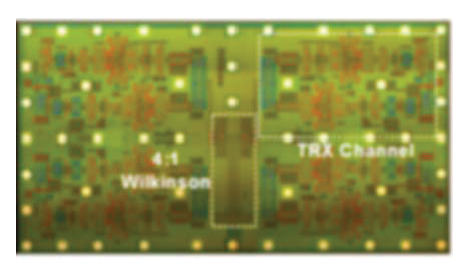
\includegraphics[width=50mm]{figures/fig_2a.eps}
		\label{fig:lores-photo}
	}%
	\\[-0.1mm]%
	\subfloat[]{%
		\centering
		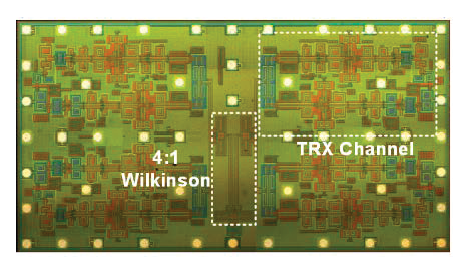
\includegraphics[width=50mm]{figures/fig_2b.eps}
		\label{fig:hires-photo}
	}%
	\\[2.6mm]
	\caption{Image resolution: (a) unacceptable; (b) acceptable.}
\end{figure}

\begin{figure*}[b]
	\centering
	\includegraphics[width=75mm]{figures/bird_1000W.eps}
	\caption{A figure which spans two columns must be placed either at the top of a page or at the bottom of a page. Figure caption with more than one line must be
		justified. Figure caption with only one line must be centered.}
	\label{fig:bird}
\end{figure*}

%%%%%%%%%%%%%%%%%%%%%%%%%%%%%%%%%%%%%%%%%%%%%%%%%%%%%%%%%%%%%%%%%%%%%%%%%%%%%

\subsection{Figure Numbers and Table Numbers}

Figures and tables must be numbered using Arabic numerals (e.g., 1, 2,
etc).

Figures have their own sequence of numbers starting from Fig. 1.
Figures must be numbered consecutively in the order they appear in
your paper.

Tables have their own sequence of numbers starting from Table 1.
Tables must be numbered consecutively in the order they appear in your
paper.

%%%%%%%%%%%%%%%%%%%%%%%%%%%%%%%%%%%%%%%%%%%%%%%%%%%%%%%%%%%%%%%%%%%%%%%%%%%%%

\subsection{Figure Captions and Table Captions}

Captions must be in 8pt regular font. A single-line caption must be
centered (e.g., Fig. 2, Table 2) whereas a multi-line caption must be
justified (e.g., Fig. 1, Fig. 3, Table 1).

A figure caption must be placed below the associated figure whereas a
table caption must be placed above the associated table.

A caption must be kept together with its associated figure or table,
i.e., they must not be separated into different columns or onto
different pages.

%%%%%%%%%%%%%%%%%%%%%%%%%%%%%%%%%%%%%%%%%%%%%%%%%%%%%%%%%%%%%%%%%%%%%%%%%%%%%

\subsection{Page Numbers, Headers and Footers}

Page numbers, headers and footers must not be used.

%%%%%%%%%%%%%%%%%%%%%%%%%%%%%%%%%%%%%%%%%%%%%%%%%%%%%%%%%%%%%%%%%%%%%%%%%%%%%

\subsection{Links and Bookmarks}

During the processing of papers for publication, all hypertext links
and section bookmarks will be removed from papers and the affected
text will be changed to black color. If you need to refer to an
Internet email address or URL in your paper, you must write the
address or URL fully in your text in regular font style and black
color.

%%%%%%%%%%%%%%%%%%%%%%%%%%%%%%%%%%%%%%%%%%%%%%%%%%%%%%%%%%%%%%%%%%%%%%%%%%%%%

\subsection{Equations}

Equations should be centered in the column and numbered sequentially.
Place the equation number to the right of the equation within a parenthesis, with
right justification within its column. An example would be

\begin{equation}
	\oint E \cdot dL = - \frac{\partial}{\partial t} \iint B \cdot dS
\end{equation}
or
\begin{equation}
	\nabla \times H = J + \frac{\partial D}{\partial t}.
\end{equation}

Note that a period is used to properly punctuate the previous
sentence.  It is placed at the end of the second equation. Make sure
that all parts of your equations are legible and are not too small to
read. When referring to an equation, use the number within
parenthesis. For example, you would usually refer to the second
equation as ``(2)'' rather than ``equation (2)''.

{% enclose the table in a group so that any redefinitions are automatically
% undone at the end of the group.
% This table has carefully handcrafted format to make it resemble its 
% sibling in the MS-WORD version of the template.
\setlength{\tabcolsep}{1mm}%
\newcommand{\CPcolumnonewidth}{50mm}%
\newcommand{\CPcolumntwowidth}{91mm}%
\newcommand{\CPcell}[1]{\hspace{0mm}\rule[-0.3em]{0mm}{1.3em}#1}%
\newcommand{\CPcellbox}[1]{\parbox{90mm}{\hspace{0mm}\rule[-0.3em]{0mm}{1.3em}#1\strut}}%
\begin{table*}
	\caption{Main predefined styles in WORD.  A Table that spans 2 columns must be placed either at top of a page or at bottom of a page.}
	\small% need this to get the 9pt text size in table cells
	\centering
	\begin{tabular}{|l|l|}\hline
		\parbox{\CPcolumnonewidth}{\CPcell{\bfseries Style Name}} & \parbox{\CPcolumntwowidth}{\CPcell{\bfseries To Format \ldots}}             \\ \hline
		\CPcell{IMS Title}                                        & \CPcell{title}                                                              \\ \hline
		\CPcell{IMS Author Block}                                 & \CPcell{author name, author affiliation, author email address}              \\ \hline
		\CPcell{IMS Author Block + Superscript}                   & \CPcellbox{affiliation marker or email address marker after an author name, \\ marker before an affiliation or an email address} \\ \hline
		\CPcell{IMS Abstract/Keywords}                            & \CPcell{abstract, keywords}                                                 \\ \hline
		\CPcell{IMS Abstract/Keywords + Italic}                   & \CPcell{abstract section heading, keywords section heading}                 \\ \hline
		\CPcell{IMS Heading 1}                                    & \CPcell{1st level section heading}                                          \\ \hline
		\CPcell{IMS Heading 2}                                    & \CPcell{2nd level section heading}                                          \\ \hline
		\CPcell{IMS Heading 3}                                    & \CPcell{3rd level section heading}                                          \\ \hline
		\CPcell{IMS Paragraph}                                    & \CPcell{paragraph}                                                          \\ \hline
		\CPcell{IMS Figure}                                       & \CPcell{figure to be centered}                                              \\ \hline
		\CPcell{IMS Figure Label}                                 & \CPcell{label placed below a component of a figure, e.g., (a) in Fig.2}     \\ \hline
		\CPcell{IMS Caption Single-Line}                          & \CPcell{figure or table caption containing one line}                        \\ \hline
		\CPcell{IMS Caption Multi-Lines}                          & \CPcell{figure or table caption containing more than one line}              \\ \hline
		\CPcell{IMS Ack/Ref Heading}                              & \CPcell{acknowledgment section heading, references section heading}         \\ \hline
		\CPcell{IMS Reference Item}                               & \CPcell{reference item}                                                     \\ \hline
	\end{tabular}
	\label{tab:wordstyles}
\end{table*}
}

%%%%%%%%%%%%%%%%%%%%%%%%%%%%%%%%%%%%%%%%%%%%%%%%%%%%%%%%%%%%%%%%%%%%%%%%%%%%%

\subsection{References}

The heading of the References section must not be numbered. All
reference items must be in 8pt font. Number the reference items
consecutively in square brackets (e.g., [1]).

When referring to a reference item, simply use the reference number,
as in [2]. Do not use ``Ref. [3]'' or ``Reference [3]'' except at the
beginning of a sentence, e.g., ``Reference [3] shows \ldots''. Multiple
references are each numbered with separate brackets (e.g., [2], [3],
[4]--[6]).

Examples of reference items of different categories shown in the
References section include the following:

\begin{itemize}
	\item	example of a book in \cite{IEEEexample:book}
	\item	example of a book in a series in \cite{IEEEexample:bookwithseriesvolume}
	\item	example of a journal article in \cite{IEEEexample:article_typical}
	\item	example of a conference paper in \cite{IEEEexample:confwithpaper}
	\item	example of a patent in \cite{IEEEexample:uspat}
	\item	example of a website in \cite{IEEEexample:IEEEwebsite}
	\item	example of a web page in \cite{IEEEexample:shellCTANpage}
	\item	example of a databook as a manual in \cite{IEEEexample:motmanual}
	\item	example of a datasheet in \cite{IEEEexample:datasheet}
	\item	example of a master's thesis in \cite{IEEEexample:masterstype}
	\item	example of a technical report in \cite{IEEEexample:techreptype}
	\item	example of a standard in \cite{IEEEexample:standard}.
\end{itemize}

%%%%%%%%%%%%%%%%%%%%%%%%%%%%%%%%%%%%%%%%%%%%%%%%%%%%%%%%%%%%%%%%%%%%%%%%%%%%%

\subsection{Balancing Columns on a Page}

There is no requirement to balance both columns on any page including
the last page, i.e., both columns are not required to be vertically
aligned at the bottom. Do not change the vertical spacing to align the
bottoms of both columns.

%%%%%%%%%%%%%%%%%%%%%%%%%%%%%%%%%%%%%%%%%%%%%%%%%%%%%%%%%%%%%%%%%%%%%%%%%%%%%

\section{Review Submission vs. Final Submission}

For review submission, in addition to other requirements, the
	{\bfseries\itshape IMS double-blind reviewing policy requires that
		all author details and the acknowledgment section be hidden.}
For final submission, you must ensure that all text which has been
hidden for review submission is unhidden.  Section V and section VI
provide hints on how to hide and unhide information in LaTeX and WORD
respectively.

%%%%%%%%%%%%%%%%%%%%%%%%%%%%%%%%%%%%%%%%%%%%%%%%%%%%%%%%%%%%%%%%%%%%%%%%%%%%%

\section{Information for LaTeX Users Only}

\subsection{Information to Hide for Review Submission}

To hide text for blind review submission, please ensure that the following
two lines in the .tex file appear uncommented and commented as shown
below:\\
\hspace*{\parindent}\parbox[t]{2in}{%
{\textbackslash}IMSthispaperforblindreview\\
$\cdots$\\
\% {\textbackslash}IMSthispaperforfinalpublication\strut
}

\subsection{Information to Unhide for Final Submission}

For final submission, you must ensure that all text which has been
hidden for blind review submission is visible by commenting the following
two lines as shown:

\noindent\hspace*{\parindent}\parbox[t]{2in}{%
\% {\textbackslash}IMSthispaperforblindreview\\
$\cdots$\\
{\textbackslash}IMSthispaperforfinalpublication
}

\subsection{All Other Must-Reads}

There are important differences between the IEEE format and the IMS
format, so you must use all files provided in the IMS LaTeX template.

If the appearance is different from what is shown in this template,
then the cause may be the use of conflicting style files in your .tex
file (e.g., latex8.sty).  You must remove all such conflicting style
files.

For the table caption to appear above the table, you must place the
table caption at the start of the table definition and before the
table cells in your .tex file.

% Example to demonstrate how to make the caption appear above the table data:
% \begin{table}
% \caption{My table caption}
% \begin{tabular}{lll}
%   ... my table cells here ...
% \end{tabular}
% \end{table}

Authors must use the {\textbackslash}raggedbottom option (as used in
this template file) to avoid LaTeX inserting inconsistent and
sometimes large spacing around section headings, around captions and
around paragraphs.

You must follow the formats as shown in this template.  You must not
use alternative styles which are not used in this template (e.g.
two-author block).

%%%%%%%%%%%%%%%%%%%%%%%%%%%%%%%%%%%%%%%%%%%%%%%%%%%%%%%%%%%%%%%%%%%%%%%%%%%%%

\section{Information for WORD Users Only}

\subsection{Information to Hide for Review Submission}

To hide text for blind review submission, select the text to be
hidden, left click to select the ``Font'' panel, and then check
``Hidden'' under the heading ``Effects''. {\bfseries\itshape To keep
the page layout unchanged, for each hidden line, you must insert one
blank line using the same style as that of the hidden text.}

\subsection{Information to Unhide for Final Submission}

For final submission, you must ensure that all text which has been
hidden for blind review submission is unhidden. Simply select the
entire WORD file, left click to select the ``Font'' panel, and then
uncheck ``Hidden'' under the heading ``Effects''.  Remove all blank
lines you have inserted as placeholders for the hidden text.

\subsection{All Other Must-Reads}

You must use the styles in Table 2 to format your paper.  To format
using a style name, open the ``Styles'' task pane under ``Home'',
select the text to be formatted, then select an appropriate style in
the ``Styles'' task pane.

When the heading styles in Table 2 are used (e.g., ``IMS Heading 1''
style), section numbers are no longer required to be typed in because
they will be automatically numbered by WORD. Similarly, reference
items will be automatically numbered by WORD when the ``IMS Reference
Item'' style is used.

Section headings must not be in all uppercase. Capitalize the headings
and then format them using an appropriate style from Table 2.

Caption width must be the same as the column width or the page width
excluding the margins. You must type the caption as a separate new
paragraph and then format the caption using an appropriate style from
Table 2. Captions must not be placed into a table or a text box
because it is difficult to set the caption width correctly within
these structures. For the same reason, insert caption command, group
command or other similar commands must not be used.

Reference items must not be formatted as a table. You must use the
appropriate styles from Table 2 to format the reference items.

After changing from single column format to two column format (e.g.
after Table 2), always make sure that both the column width and the
column spacing are the same as specified in the last paragraph of
section II.B.

If your WORD document contains equations, you must not save your WORD
document from ``.docx'' to ``.doc'' because when doing so, WORD will
convert all equations to images of unacceptably low resolution.

%%%%%%%%%%%%%%%%%%%%%%%%%%%%%%%%%%%%%%%%%%%%%%%%%%%%%%%%%%%%%%%%%%%%%%%%%%%%%

\section{Conclusion}

The format of this template was adapted by Causal Productions mainly
from the IEEE LaTeX class file. There are important differences
between the IEEE format and the IMS format, so IMS authors must use
only the latest version of the IMS templates.

IMS offers US Letter templates for LaTeX and WORD. The version of
this template is V6. Changes from V5 to V6 are:

\begin{itemize}
	\item	page limit in section II.A, including updated information on page
	      formatting requirements for final papers for proceedings or MWTL submission
	\item For LaTeX version, show LaTeX double-blind instructions first
	\item	For WORD version, show WORD double-blind instructions first
	\item	list of changes from previous version to current version.
\end{itemize}

%%%%%%%%%%%%%%%%%%%%%%%%%%%%%%%%%%%%%%%%%%%%%%%%%%%%%%%%%%%%%%%%%%%%%%%%%%%%%

\section*{Acknowledgment}

% the following macro \IMSdisplayacksection makes its argument visible for the
% final paper, but hides its argument for the blind-review paper while keeping
% a blank vertical space of the same size.  The actual text of the acknowledgement
% is defined inside the macro \IMSacktext so that multiple paragraphs will be
% displayed or hidden correctly.

\newcommand{\IMSacktext}{%
	The headings of the Acknowledgment section and the References section
	must not be numbered.

	Causal Productions wishes to acknowledge Michael Shell and other
	contributors for developing and maintaining the IEEE LaTeX class file
	used in the preparation of this template.  To see the list of
	contributors, please refer to the top of file IEEETran.cls in the IEEE
	LaTeX distribution.
}

\IMSdisplayacksection{\IMSacktext}% end of \IMSdisplayacksection

%%%%%%%%%%%%%%%%%%%%%%%%%%%%%%%%%%%%%%%%%%%%%%%%%%%%%%%%%%%%%%%%%%%%%%%%%%%%%

\bibliographystyle{IEEEtran}

\bibliography{IEEEabrv,IEEEexample}

\end{document}

